\documentclass[11pt,a4paper]{article}

%include polycode.fmt

\usepackage[margin=2.5cm]{geometry}
\usepackage{todonotes}
\usepackage{microtype}
\usepackage{listings}
\usepackage{color}
\usepackage{amssymb,amsmath}
\usepackage{mathpazo}
\usepackage{accents}
\usepackage{longtable,booktabs}
\usepackage{dcolumn}
\usepackage{pgf}
\usetikzlibrary{shapes.geometric}
\usetikzlibrary{matrix}
\usepackage{natbib}
\usepackage{hyperref}
\usepackage[capitalise,noabbrev,nameinlink]{cleveref}
\hypersetup{
  pdftitle={Pipelining in Ouroboros chain diffusion},
  pdfborder={0 0 0},
  breaklinks=true
}

\definecolor{dkgreen}{rgb}{0,0.6,0}
\definecolor{gray}{rgb}{0.5,0.5,0.5}
\definecolor{pink}{rgb}{0.92,0.2,0.86}

\lstset{frame=tb,
  language=Haskell,
  aboveskip=3mm,
  belowskip=3mm,
  showstringspaces=false,
  columns=flexible,
  basicstyle={\small\ttfamily},
  numbers=none,
  numberstyle=\tiny\color{pink},
  keywordstyle=\color{pink},
  commentstyle=\color{pink},
  stringstyle=\color{pink},
  breaklines=true,
  breakatwhitespace=true,
  tabsize=3
}

\DeclareMathOperator{\dom}{dom}
\newcommand\restrict[2]{\left.#1\right||_{#2}}
\newcommand\deltavar[1]{\accentset{\Delta}{#1}}

\begin{document}

\title {Pipelining in Ouroboros chain diffusion\\
       {\large \sc An IOHK discussion paper / high level design}}
\date  {Version 0.4, 19th January 2022}
\author{Duncan Coutts      \\ {\small \texttt{duncan@well-typed.com}} \\
                              {\small \texttt{duncan.coutts@iohk.io}} \\
   \and Matthias Fitzi     \\ {\small \texttt{matthias.fitzi@iohk.io}} \\
   \and John Woods         \\ {\small \texttt{john.woods@iohk.io}} \\
                              {\small \texttt{john@postquantum.dev}} \\
}

\maketitle

\section{Purpose}
The purpose of this document is to present a proposed change to the algorithm
for Ouroboros chain diffusion that, if implemented, could facilitate higher block validation times
for the same choice of the $\Delta$~diffusion time.
Ergo, we would enjoy a faster $\Delta$~diffusion time in the context of our current block validation requirements.
This additional budget may be spent on increasing block-size, and/or increasing CPU \& memory limits for Plutus scripts.
This document will attempt to analyse the algorithm, and review its implications. The document also discusses which 
implementation changes would be necessary to execute the change in practice.

\pagebreak

\tableofcontents

\pagebreak

\section{Acknowledgements}
The ideas presented herein are inspired by and based on discussions with several
people from the research and engineering groups: Giorgos Panagiotakos,
Sandro Coretti-Drayton, Karl Knutsson, Marcin Szamotulski, Nick Frisby,
Neil Davies, Peter Thompson and Philipp Kant.

\section{Context}
Whilst the research team have been considering the design for Ouroboros Leios
(using input endorsers), the process has spawned some ideas for potential changes to
the existing Ouroboros Praos algorithm, which may also result in a more uniform (and therefore
more efficient) use of a node's network and CPU resources. In discussion with engineering, both 
Network and Consensus teams, these ideas multiplied into a range of plausible options.

A particularly radical idea, referred to by research as "heretic pipelining" (read: aggressive), is 
a pipelined augmentation of the Praos algorithm which requires that we handle invalid/partially invalid blocks.
Predicated on the notion that under Ouroboros Praos, the higher the density of a chain the 
harder it is to attack, the contention should hold that we may want to permit "invalid" or "partially 
invalid" blocks to be added to the chain, should they be produced by validly elected slot leaders.
This would ensure that the chain density doesn't suffer during pipelining (which would make the chain 
weaker and more susceptible to attack), whilst we still enjoy the benefits of aggressive pipelining.

In this document however, we will only present the least radical of the evoked ideas, 
i.e. \emph{non-aggressive} diffusion pipelining, that we believe would involve the fewest changes to the 
design/implementation, without the need to handle invalid blocks, yet that nevertheless, may provide a substantial benefit.

\section{Introduction}
The key idea is to diffuse block bodies \emph{before} having fully validated
them. This takes the block body validation work out of the \emph{critical path} of
block diffusion. It permits the validation time spent on each 'hop' in the path to be
overlapped with sending the block on to the next node in the path.

On the presumption that there are typically $N$ hops in the path during block diffusion
within the Cardano network, and block body validation takes $V$ seconds, then in
principle this change could save $(N-1) V$ seconds overall diffusion time. Equivalently, 
instead of having to fit $N$ validations into the $\Delta$ time budget, we need 
only fit ~$1$. This makes more efficient use of the $\Delta$ time budget, this excess 
of time can in-turn be used to increase the block-size and/or allow for an increase of 
the block validation time (such as to permit execution of longer running scripts,
enabled by increases to the Plutus abstract CPU \& memory unit limits).

\pagebreak

\section{The existing block relaying scheme}
The main steps followed by each node, on the critical path of block relay, flow approximately
as follows:

\begin{enumerate}
  \item Request and transmit the block header (from the upstream peer);
  \item Validate the block header;
  \item Request and transmit the block body (from the upstream peer);
  \item Validate the block body and extend the local chain;
  \item Transmit the block header (to downstream peers);
  \item Transmit the block body (to downstream peers);
\end{enumerate}

On a stylized time-line (with time running from left to right), we can depict
this as:

\begin{center}
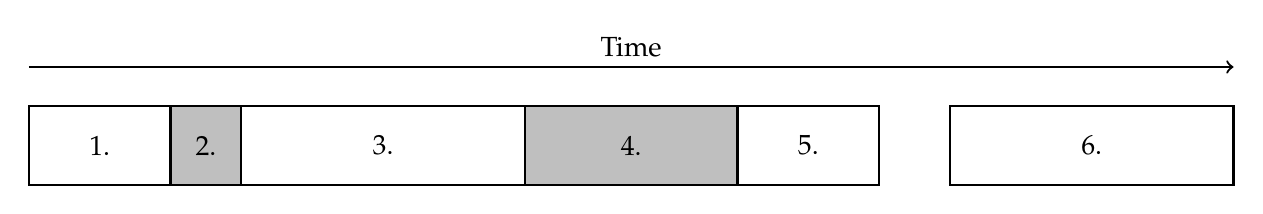
\begin{tikzpicture}
\begin{scope}[thick, xscale=0.9]

\draw (0,0) rectangle (2,1);
\draw[fill=lightgray] (2,0) rectangle (3,1);
\draw (3,0) rectangle (7,1);
\draw[fill=lightgray] (7,0) rectangle (10,1);
\draw (10,0) rectangle (12,1);
\draw (13,0) rectangle (17,1);

\draw (1,  0.5) node {1.};
\draw (2.5,0.5) node {2.};
\draw (5,  0.5) node {3.};
\draw (8.5,0.5) node {4.};
\draw (11, 0.5) node {5.};
\draw (15, 0.5) node {6.};

\draw[->] (0, 1.5) -- (17, 1.5);
\draw     (8.5, 1.5) node[anchor=south] {Time};

\end{scope}
\end{tikzpicture}
\end{center}

Of course, this represents a single hop in the broader picture of block propagation and in a network there will typically
be 5 -- 7 such hops between a given block producer, and the last block producer in the path. In the current design we 
fully validate blocks before relaying them, so the overall time-line looks like this:

\begin{center}
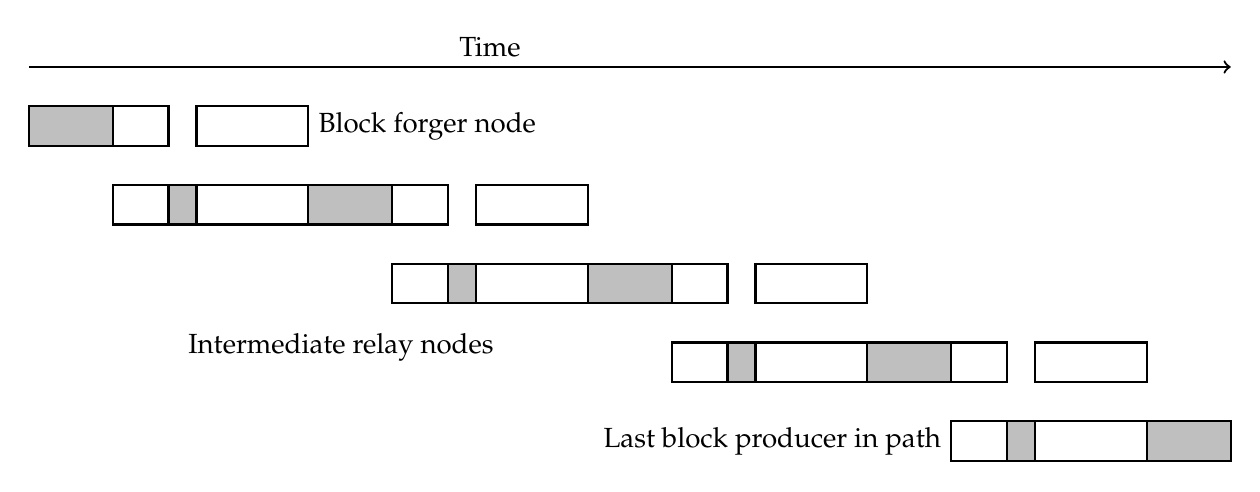
\begin{tikzpicture}
\begin{scope}[thick, xscale=0.355, yscale=0.5]

\begin{scope}
  \draw[fill=lightgray] (7,0) rectangle (10,1);
  \draw (10,0) rectangle (12,1);
  \draw (13,0) rectangle (17,1);
  \draw (17, 0.5) node[anchor=west] {Block forger node};
\end{scope}

\begin{scope}[xshift=10cm, yshift=-2cm]
  \draw (0,0) rectangle (2,1);
  \draw[fill=lightgray] (2,0) rectangle (3,1);
  \draw (3,0) rectangle (7,1);
  \draw[fill=lightgray] (7,0) rectangle (10,1);
  \draw (10,0) rectangle (12,1);
  \draw (13,0) rectangle (17,1);
\end{scope}

\begin{scope}[xshift=20cm, yshift=-4cm]
  \draw (0,0) rectangle (2,1);
  \draw[fill=lightgray] (2,0) rectangle (3,1);
  \draw (3,0) rectangle (7,1);
  \draw[fill=lightgray] (7,0) rectangle (10,1);
  \draw (10,0) rectangle (12,1);
  \draw (13,0) rectangle (17,1);
  \draw (4, -0.5) node[anchor=north east] {Intermediate relay nodes};
\end{scope}

\begin{scope}[xshift=30cm, yshift=-6cm]
  \draw (0,0) rectangle (2,1);
  \draw[fill=lightgray] (2,0) rectangle (3,1);
  \draw (3,0) rectangle (7,1);
  \draw[fill=lightgray] (7,0) rectangle (10,1);
  \draw (10,0) rectangle (12,1);
  \draw (13,0) rectangle (17,1);
\end{scope}

\begin{scope}[xshift=40cm, yshift=-8cm]
  \draw (0,0) rectangle (2,1);
  \draw[fill=lightgray] (2,0) rectangle (3,1);
  \draw (3,0) rectangle (7,1);
  \draw[fill=lightgray] (7,0) rectangle (10,1);
  \draw (0, 0.5) node[anchor=east] {Last block producer in path};
\end{scope}

\draw[->] (7, 2) -- (50, 2);
\draw     (23.5, 2) node[anchor=south] {Time};

\end{scope}
\end{tikzpicture}
\end{center}

\pagebreak

\section{The proposed block relaying scheme}
By propagating forward a block as soon as it has arrived locally (and its header is validated), the block 
validation time is overlapped with the propagation time and the overall timeline becomes materially shorter.

\begin{center}
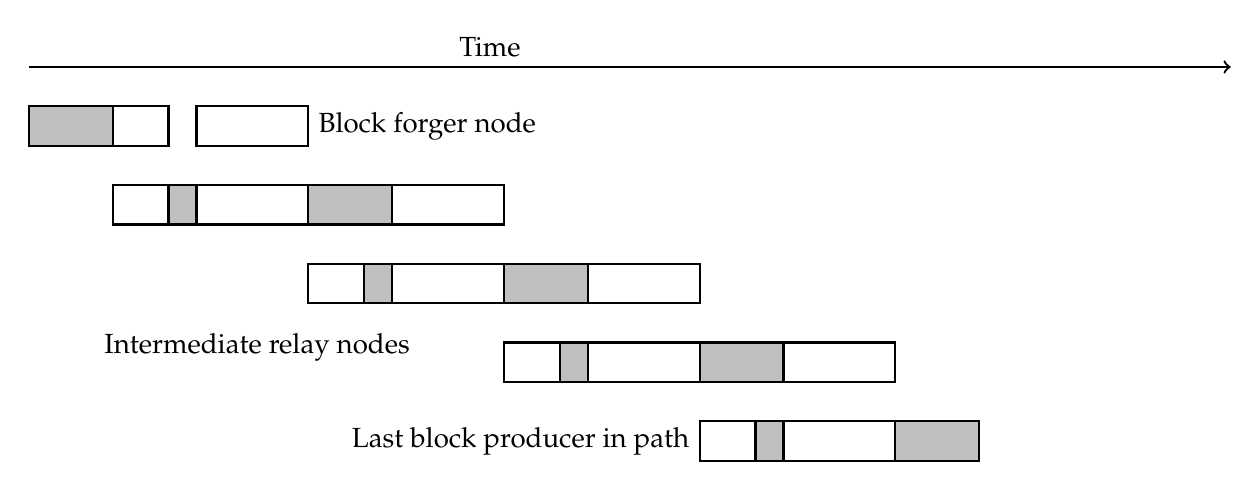
\begin{tikzpicture}
\begin{scope}[thick, xscale=0.355, yscale=0.5]

\begin{scope}
  \draw[fill=lightgray] (7,0) rectangle (10,1);
  \draw (10,0) rectangle (12,1);
  \draw (13,0) rectangle (17,1);
  \draw (17, 0.5) node[anchor=west] {Block forger node};
\end{scope}

\begin{scope}[xshift=10cm, yshift=-2cm]
  \draw (0,0) rectangle (2,1);
  \draw[fill=lightgray] (2,0) rectangle (3,1);
  \draw (3,0) rectangle (7,1);
  \draw[fill=lightgray] (7,0) rectangle (10,1);
  \draw (10,0) rectangle (14,1);
\end{scope}

\begin{scope}[xshift=17cm, yshift=-4cm]
  \draw (0,0) rectangle (2,1);
  \draw[fill=lightgray] (2,0) rectangle (3,1);
  \draw (3,0) rectangle (7,1);
  \draw[fill=lightgray] (7,0) rectangle (10,1);
  \draw (10,0) rectangle (14,1);
  \draw (4, -0.5) node[anchor=north east] {Intermediate relay nodes};
\end{scope}

\begin{scope}[xshift=24cm, yshift=-6cm]
  \draw (0,0) rectangle (2,1);
  \draw[fill=lightgray] (2,0) rectangle (3,1);
  \draw (3,0) rectangle (7,1);
  \draw[fill=lightgray] (7,0) rectangle (10,1);
  \draw (10,0) rectangle (14,1);
\end{scope}

\begin{scope}[xshift=31cm, yshift=-8cm]
  \draw (0,0) rectangle (2,1);
  \draw[fill=lightgray] (2,0) rectangle (3,1);
  \draw (3,0) rectangle (7,1);
  \draw[fill=lightgray] (7,0) rectangle (10,1);
  \draw (0, 0.5) node[anchor=east] {Last block producer in path};
\end{scope}

\draw[->] (7, 2) -- (50, 2);
\draw     (23.5, 2) node[anchor=south] {Time};

\end{scope}
\end{tikzpicture}
\end{center}

Alternatively, this saving can be used to substantially increase the time available for
block validation, or indeed for propagation of larger blocks, as shown below:

\begin{center}
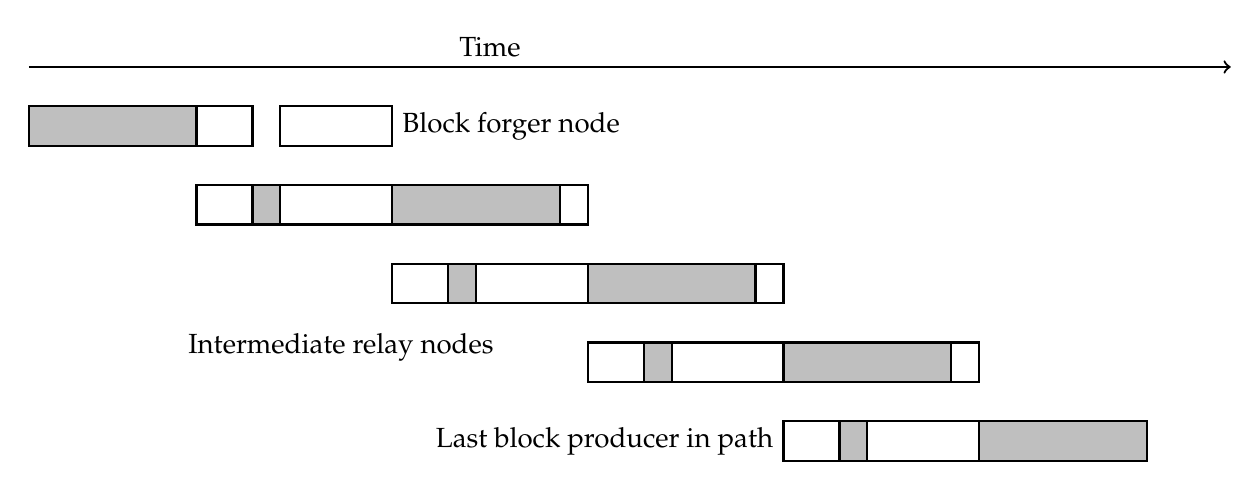
\begin{tikzpicture}
\begin{scope}[thick, xscale=0.355, yscale=0.5]

\begin{scope}
  \draw[fill=lightgray] (7,0) rectangle (13,1);
  \draw (13,0) rectangle (15,1);
  \draw (16,0) rectangle (20,1);
  \draw (20, 0.5) node[anchor=west] {Block forger node};
\end{scope}

\begin{scope}[xshift=13cm, yshift=-2cm]
  \draw (0,0) rectangle (2,1);
  \draw[fill=lightgray] (2,0) rectangle (3,1);
  \draw (3,0) rectangle (7,1);
  \draw[fill=lightgray] (7,0) rectangle (13,1);
  \draw (13,0) rectangle (14,1);
\end{scope}

\begin{scope}[xshift=20cm, yshift=-4cm]
  \draw (0,0) rectangle (2,1);
  \draw[fill=lightgray] (2,0) rectangle (3,1);
  \draw (3,0) rectangle (7,1);
  \draw[fill=lightgray] (7,0) rectangle (13,1);
  \draw (13,0) rectangle (14,1);
  \draw (4, -0.5) node[anchor=north east] {Intermediate relay nodes};
\end{scope}

\begin{scope}[xshift=27cm, yshift=-6cm]
  \draw (0,0) rectangle (2,1);
  \draw[fill=lightgray] (2,0) rectangle (3,1);
  \draw (3,0) rectangle (7,1);
  \draw[fill=lightgray] (7,0) rectangle (13,1);
  \draw (13,0) rectangle (14,1);
\end{scope}

\begin{scope}[xshift=34cm, yshift=-8cm]
  \draw (0,0) rectangle (2,1);
  \draw[fill=lightgray] (2,0) rectangle (3,1);
  \draw (3,0) rectangle (7,1);
  \draw[fill=lightgray] (7,0) rectangle (13,1);
  \draw (0, 0.5) node[anchor=east] {Last block producer in path};
\end{scope}

\draw[->] (7, 2) -- (50, 2);
\draw     (23.5, 2) node[anchor=south] {Time};

\end{scope}
\end{tikzpicture}
\end{center}

\pagebreak

\section{Risk analysis}
Before we analyse the risks it is important to be precise about which validations
will still be executed as normal, and which would be deferred. The following are
validations which should still be done:

\begin{enumerate} 
  \item The hash validation to ensure that the block body content matches the header;
  \item Nodes relaying blocks would only relay a single block in advance of validating the block body; and
  \item Block producers would still validate the block body before creating a new block.
\end{enumerate}

\emph{Thus, the only validation which is deferred is that on the block body content.}

\section{Analysis of DoS risks}
The immediate concern is whether executing less prompt validation would
create any new opportunities for denial-of-service attacks. In general the reason
we take a very conservative approach to chain diffusion -- in which we validate
fully and promptly -- is to avoid denial-of-service attacks. The general
principle has been that whilst we have found ways to bound the amount of work
honest nodes need to do for valid block data, it is substantially harder to
bound work if we propagate invalid data.

That said, the goal is not to prevent invalid data from being relayed over the
network graph. The goal is to prevent honest nodes from being required to do an
unbounded amount of work, and indeed more stringently, to prevent honest nodes
from having to do more work than the dishonest nodes engaged in an attack. Thus,
if we can relax or defer validation without increasing the work compared with the
normal valid case, then the risk may be acceptable. In particular, we need to avoid any
situations whereby previously we executed a single expensive step, and now we would do many.

The combination of checks 1.~and 2.~above should mean that the possibly-invalid
block is one which was signed by the block producer (KES validation), who (in-turn) was
authorised to create a block in this slot (VRF verification). This should mean that
there cannot be a greater number of invalid blocks, in total, than in the case of valid blocks. In
particular intermediate nodes cannot forge any extra or altered block(s) without
falling afoul of these checks. Thus, it should be the case that only the
authorised block producer can create many valid blocks, or many valid block
headers with invalid block bodies.

\pagebreak

\subsection{Many valid block headers}
\label{many-valid-block-headers}
As noted above, it is already possible for authorised block producers to sign
many valid blocks in their slot. It is instructive to see how we can avoid
honest nodes doing an unbounded amount of work in this situation.

Suppose one or more adversarial nodes are slot leaders (e.g. in recent slots)
and they extend the current chain with multiple different but \emph{valid}
blocks. They could each create multiple blocks individually, or collaborate to
extend each other's chains. Either way, the chains will differ only in the final
few blocks. Now suppose an honest node becomes aware of many of these different
chains (e.g. from different peers). The honest node will validate and adopt the
first chain it manages to download (though it will try to pick the longest (densest) first).
The question then is whether the honest node would stop there or if it would be
persuaded to adopt a bounded or an unbounded number of the alternative chains.

Chains are ordered by the chain selection algorithm. Chains will only be adopted if
they are strictly better in that ordering. The ordering is the lexicographic
combination of:

\begin{enumerate}
  \item Order by chain length (longer chains preferred);
  \item If the last block slot numbers are the same then order by whether \emph{this} node produced the block or not (locally produced blocks preferred);
  \item If the last blocks were issued by the same entity (same SPO cold key), then order by the hot key certificate issue number (higher cert issue number preferred);
  \item Finally, order by VRF value (lower VRF value preferred).
\end{enumerate}

An appropriate way to analyse this is to argue that there can only be bounded
progress in this order.

\begin{enumerate}
  \item In the short term, the chain length is bounded by the Ouroboros leader schedule.
  \item The second condition is boolean, so it is bounded.
  \item The certificate counters are controlled by the block issuers and are not inherently bounded. This needs special treatment to establish a bound.
  \item The VRF value depends on the identity of the block issuer, but its value is not under the issuer's control. We rely on the property of the VRF primitive that it's only possible to create a single valid value per block issuer, per slot. Given this, the number of different VRF values is bounded by the number of different authorised block issuers (from the end of the most recent common chain) which is then bounded by the Ouroboros leader schedule.
\end{enumerate}

\emph{So the only case that needs special treatment is bounding the certificate issue numbers.} \\

The purpose of the certificate issue numbers is to enable a block producer to
cycle their hot keys and in particular to be able to issue a new hot key if the
current hot key is compromised. The reason one might compare on certificate issue
numbers at all is in the situation where a compromised hot key is being used
to sign blocks. In this situation the true owner needs to issue a new hot key
with a new, higher certificate issue number, via their cold key, and then 
use that new hot key to sign blocks. 

This results in the possibility that the stolen key and the new key (with corresponding certs) 
may be being used at the same time, and they have to compete to be selected. This is why the 
chain selection rule prefers the later issue number, so it will be selected even if the block 
signed by the compromised key arrives first and is thus selected first.

In principle the certificate issue numbers are not bounded, but the use case
of recovering from compromised keys does not require more than two issue
numbers. So 'progress' in the certificate issue number can be bounded by
allowing at most two different blocks with the same issuer in the same slot.
There is also a 'no regression' rule with regard to the issue numbers used on the chain, so
even if an attacker has several compromised certificates, as soon as they
use a later one, then the earlier ones can no longer be used again.

\subsection{Many valid block bodies}
The case for many block bodies is straightforward: they make no difference to
chain selection. So there being multiple different blocks with different
content does not alter the informal argument above. It is certainly adversarial
behaviour for a single block producer to create multiple different blocks in a
slot, but it does not directly create more work for the honest nodes. A node that
has adopted a chain, will not select another from the same producer since it is not
better from a chain selection ordering perspective.

\subsection{Many invalid block bodies}
\label{many-invalid-block-bodies}
If we postpone block body validation in the way proposed herein, then all the
considerations made about "many valid blocks" still apply, and in addition we must
analyse the new cases for invalid block bodies. For this part of the analysis
we can presume that the block header is valid.

The bounding argument for the valid block case relies on making strict
progress in the chain selection ordering, and thus the overall opportunity to make
progress being bounded. The immediate difficulty in trying the same argument
with invalid block bodies is that once we discover they are invalid, and we
stick with our current chain, then we have not made any progress in the chain
selection ordering. We return to the same state where we are prepared to
consider fresh (or perhaps even the same) invalid blocks.

Under the full prompt validation model when we encounter an invalid block we
can promptly cut off all peers that gave us that invalid block (even peers
that just gave us the header). We cannot do that under the delayed block body
validation proposal because we can no longer pin the blame on the immediate
peer for failing to validate the block body before sending it to us.

Fortunately this problem does not appear insurmountable. We can still pin the
blame for a bad block on the issuer of the block. The block issuer is typically
not a direct peer therefore we cannot use disconnection as a solution. If however, we simply
employ some state to temporarily store the block issuer details, then we can use that reference
to not consider any more blocks signed by this issuer in this slot. They
have demonstrated themselves to be adversarial by signing a bad block, and we
shouldn't spend any further resources validating blocks from them in the short term. 
Note that for this purpose we must identify the block issuer by the hot key certificate and 
not the `cold' permanent identity. This is due to the fact that a compromised hot key could 
be used to sign bad blocks, and that ought to still be a situation from which a block producer can 
recover from by signing a new certificate with a higher issue number.

It appears that it would be sufficient to hold a state of bad block issuers
(identified by certificate) \emph{only until} the current chain is successfully
extended. This approach would avoid considering more than a single bad block from any
recent issuer. The number of recent adversarial issuers (and thus the size of
the tracking set) is bounded by the leadership schedule and the honest stake
assumption. The certificate counters are bounded (or can be bounded) as
described in \cref{many-valid-block-headers}.

\pagebreak

\section{Implementation changes}
The implementation changes required to deliver on the approach discussed in this document
are all to be made within the Consensus layer. The discussion in this section pertains specifically 
to the "non-aggressive" diffusion pipelining variant, the specific novel behaviour here is, nodes now
forward \emph{one unvalidated block}, so that multiple nodes can download and validate the latest 
block \emph{concurrently}. To begin, let us remind ourselves how Cardano currently diffuses data:

\begin{itemize}
  \item With Ouroboros Praos, we want the block minted in a given slot to diffuse to the leader of the next slot early enough that they in-turn can extend the chain on-top of it.
  \item With Praos, a node will adopt the chain which is most dense and whose intersection with the previous "best" known chain is less than $k$ blocks, where $k$ is currently set to 2160.
  \item Cognisant of the above, the process continues as follows:
  \begin{enumerate}
    \item A node will notify interested peers that a new block is available by posting the new header to \lstinline{chainSync}, after block validation. 
    \item After the header is validated the downstream peer will request/pull the corresponding block body.
    \item The block is validated, and if it satisfies checks resulting in a new longer/better chain, it will be appended as the head of our "new" chain.
    \item This process repeats for each downstream peer.
  \end{enumerate}
\end{itemize}

It's clear from the above description that without pipelining we incur the block validation overhead,
scaling linearly with the number of hops a block travels during its diffusion across the critical path.
Let us now consider the following implementation changes to data diffusion in the Consensus layer to achieve
a faster block propagation and adoption time with pipelining, the goal is to provide a \emph{mechanism} by which we 
can expedite a block's propagation prior to its validation whilst not invalidating existing protocol primitives:

\begin{itemize}
  \item The aim is to expedite data propagation where appropriate, and to do so without destructive change.
  \begin{enumerate}
    \item Extend the current API to pre-notify subscribed threads when a new desirable block is seen.
    \item Implement a new mini-protocol which can function as an "expedited" version of \lstinline{chainSync}.
    \item The new protocol should provide two new mechanisms:
    \begin{itemize}
      \item The ability to send a fresh block header to a downstream peer as soon as a given node witnesses a new desirable block, prior to actually validating it. This enables the downstream peer to pre-emptively fetch this new block.
      \item The ability for a downstream peer to register interest in receiving another expedited block. 
    \end{itemize}
    \item Regular sanity checks still apply:
    \begin{itemize}
      \item Ignore headers which don't extend the currently selected chain.
      \item Disconnect from a peer if a given header is invalid.
      \item Do not expedite any data which is not definitively more desirable than all previous data expedited. 
    \end{itemize} 
  \end{enumerate}
  \item Appropriately handle misbehaving peers, as per \cref{many-invalid-block-bodies}. Further discussion on this point is included in the section following, \cref{conclusion-and-considerations}.
\end{itemize}
  
\pagebreak
  
\section{Conclusion \& considerations}
\label{conclusion-and-considerations}
It appears that diffusion pipelining is an exciting and potentially highly valuable 
modification to the block propagation approach for Cardano core. There are some considerations
though which one should bear in mind during implementation:

\begin{itemize}
  \item We must of course, ensure faster than real-time syncing of the chain. This is not an issue for the proposed implementation herein, however it's something we must be cognisant of in the future.
  \item The changes proposed herein don’t affect the structural properties of the chain.
  \item Intuitively one may be inclined to suggest a change to minting policy, given that with pipelining an SPO now \emph{knows} that a potentially better chain exists to extend. However, knowledge of this reality (\emph{which existed prior to pipelining}), should not alter minting behaviour. 
  \item We should not expedite/pipeline a subsequent block until the previously pipelined block is validated, i.e. do not pipeline multiple blocks concurrently.
  \item Pipelining ultimately results in maximal use of computing resource, which may not always be desirable as said resource is needed for other functions. However, this is not a concern for this proposed non-aggressive variant.
  \item We may wish to implement logic to deal with the receipt of multiple bad blocks. As discussed above we cannot simply "cut-off" a connection to a peer, as blame cannot be levied directly at a given peer. However, we could run a check on the KES (Key-evolving Signature), which would enable us to build conditional logic to ignore blocks from a misbehaving block producer.
  \item The aggressive pipelining variant, not covered in detail herein, will require further consideration and design, such as:
  \begin{enumerate}
    \item The aggressive approach implies that our current presumptions with regard to the validity of individual blocks no longer holds.
    \item The aggressive approach will require further analysis with regard to handling pipelined blocks concurrently. 
  \end{enumerate}
\end{itemize}
\end{document}